\clearpage
\subsubsection{Record} % (fold)
\label{ssub:record}

A Record (Structure in C) is a composite type whose value is made up of a number of \textbf{fields}. Each field stores a value of a certain type. A value of the record's type stores data for each field described in the Record/Structure. 

In your code, records can be used to model data associated with the \emph{things}, the \emph{entities}, associated with your program. For example, a financial application can have records to store \texttt{Account}, \texttt{Customer}, and \texttt{Transaction} values. A murder mystery game may have \texttt{Player}, \texttt{Clue}, and \texttt{Scene} values, where as a Space Invaders game would have \texttt{Player}, \texttt{Alien}, and \texttt{Bullet} values. Each of these would be modelled in code using a Record/Structure.

\begin{figure}[h]
   \centering
   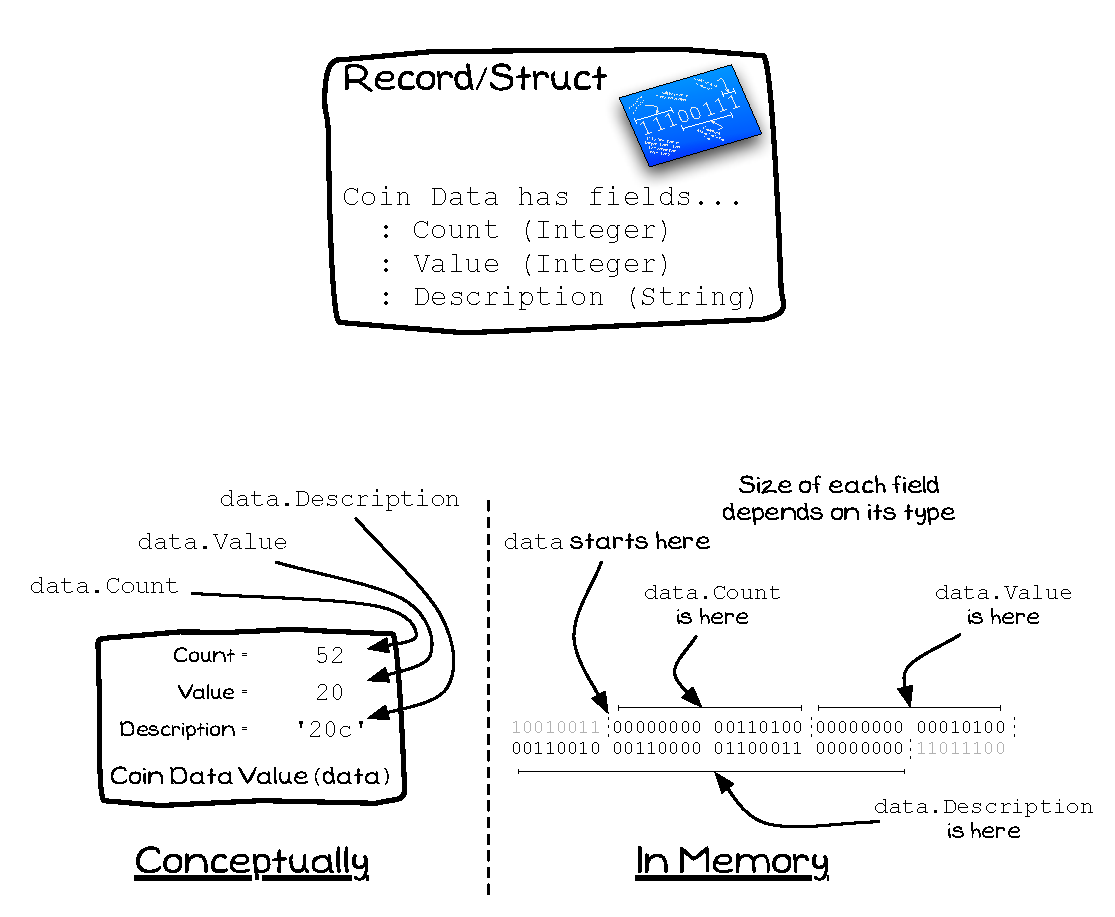
\includegraphics[width=\textwidth]{./topics/type-decl/diagrams/Record} 
   \caption{A Record or Structure contains Fields}
   \label{fig:type-decl-record}
\end{figure}

\mynote{
\begin{itemize}
  \item A Record/Structure is a kind of \textbf{artefact} you can declare.
  \item You can create your own Record/Structure types, these can then be used to define the data stored in \nameref{sub:variable}s in your code.
  \item Remember that this is declaring a new data format, it is not declaring a new data value: for that you need to declare a \nameref{sub:variable}.
  \item The \textbf{size} of a record is based on the sum of the sizes of its fields.
\end{itemize}
}

% subsection record_or_structure (end)